\chapter{Tests et analyse défauts fonctionnels ESD}
\label{chap:1}
\section{Contexte}

% What generates an ESD
Une décharge électrostatique est le résultat d'une accumulation de potentiel électrostatique, causée par induction électrique ou de la triboélectricité.
La charge triboélectrique se produit par transfert d'électrons lorsque deux objects sont mis en contact puis séparés.
Un objet se charge positivement et l'autre négativement.
Le signe de la charge dépend du matériau de l'objet.
La charge par induction se produit lorsque l'objet baigne dans un champs électrique, puis est soudainement mis à la masse.

% Electronic devices are exposed to ESD, in factories first
Les décharges électrostatiques sont un problème important pour les systèmes électroniques.
Des défaillances peuvent se produire pendant la fabrication ou pendant la vie du produit.
Pendant la fabrication, les circuits sont manipulés par des machines, ce qui cause des contacts répétés et éventuellement une accumulation de charges.
Il existe plusieurs standards de test pour garantir qu'un produit peut survivre aux étapes de fabrication.
Les testers HMM (Human Machine Model) et CDM (Charged Device Model) valident respectivement la robustesse vis-à-vis de la décharge d'un objet dans le produit, et la décharge du produit dans la masse.
Ces tests sont concus pour reproduire fidèlement les stress rencontrés dans l'environnement de fabrication.

% Electronic devices are exposed to ESD in the field
Des défaillances peuvent aussi apparaitre une fois le produit déployé sur le terrain.
Dans le cas de produits grand-public, elles peuvent être causées par la manipulation des objets par des humains chargés électriquement.
C'est le cas des téléphones portables et des caméras par exemple.
Dans l'environnement automobile, les contraintes sont encore plus fortes à cause d'autres phénomènes de génération de tribo-électricité.

% Hard-failure is one thing, soft-fail another
Il y a deux classes de défaillances dues aux ESD.
La casse matérielle est le premier type de défaillance.
Le composant est détruit après une décharge et doit être remplacé.
La perte de fonctionnalité est le second type, et se produit alors que le produit est alimenté et en fonctionnement normal.
La décharge perturbe une ou plusieurs fonctions, qui a besoin d'un délai pour récupérer.
Parfois, la fonction est bloquée et un rédemarrage manuel du produit est requis pour rétablir un fonctionnement normal.

\section{Méthodes de test ESD}

Pour reproduire les décharges électrostatiques dans un laboratoire, de multiples générateurs de test existent.
Le TLP (Transmission Line Pulser) est un des plus largement utilisés.
Il est employé dans une variété d'applications, pour la characterization de composants \cite{TLPforESDProtectionCz, TLPthroubleshooting}, l'investigation de défaillances \cite{tlp-application-1, tlp-application-2} et la correlation avec d'autre générateurs de test \cite{correlation-system-level-esd-tlp}.
Cette technique a été inventée par T. Maloney et N. Nakamura \cite{TLP}.
Elle est en cours de standardisation avec ANSI/ESD STM 5.5.1-2016 \cite{tlp-standard}.
Ce type de générateur a été longuement étudié dans les thèses de N. Monnereau \cite{phd-monnereau} et N. Lacrampe \cite{phd-lacrampe}.

% Concept
Un TLP génère une impulsion rectangulaire très courte, en utilisant la décharge d'un câble coaxial (Fig. \ref{tlp_concept}).
Le câble est initialement chargé par une source haute-tension à travers une résistance de forte valeur.
Une fois la tension du câble suffisamment élevée, un relai est commuté pour déclencher la décharge.
Le coaxial utilisé a généralement une impédance charactéristique de 50\textOmega{} et une longeur de 5 mètres, correspondant à un délai de 50ns de propagation.
La décharge produite par un tel câble est deux fois plus longue (à cause des effets de propagation) et dure 100ns.

\begin{figure}[!h]
  \centering
  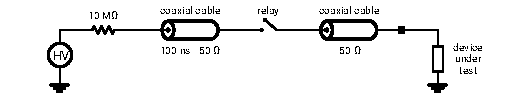
\includegraphics[width=\textwidth]{src/1/figures/tlp_concept.pdf}
  \caption{Minimal example of a \gls{tlp} system}
  \label{tlp_concept}
\end{figure}

% Characteristics of tlp systems
Un système TLP produit des impulsions très reproductibles, car l'environnement est très bien maitrisé et la décharge a lieu dans un chemin de propagation blindé et isolé des perturbations extérieures.
L'impédance characteristique de 50\textOmega{} peut être maintenue jusqu'à la charge The characteristic impedance of  can be controlled up to the load, by using appropriate 50\textOmega{} cables and hardware.
Les propriétés clés d'une impulsion TLP sont données dans la figure \ref{tlp_pulse}.

\begin{figure}[!h]
  \centering
  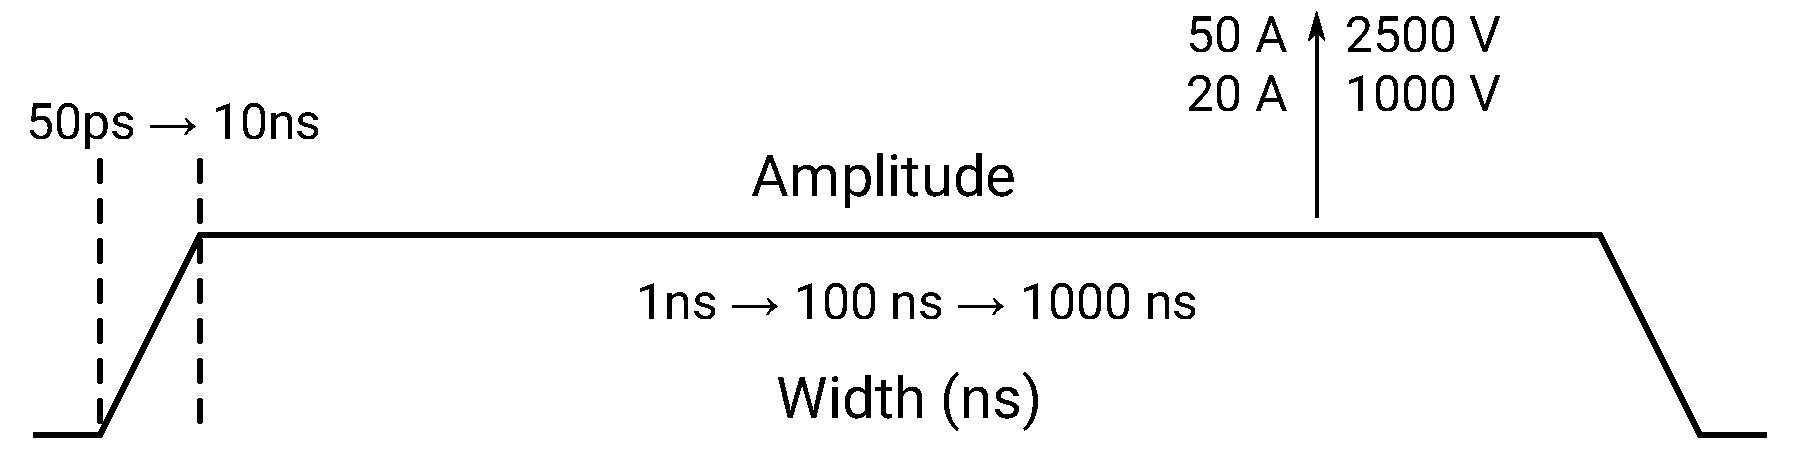
\includegraphics[width=\textwidth]{src/1/figures/tlp_pulse.pdf}
  \caption{Main characteristics of a \gls{tlp} pulse on a resistive load}
  \label{tlp_pulse}
\end{figure}

% ESD guns
Le TLP est un excellent outil de test et d'investigation, mais la forme d'onde est très différente d'une vraie décharge électrostatique.
Pour garantir la robustesse d'un produit, les pistolets de décharge ESD sont préférables.
Les standard IEC 61000-4-2 \cite{iec61000-4-2} et ISO 10605 \cite{iso10605} definissent une forme d'onde de test pour les systèmes électroniques.
Elle reproduit la décharge d'un corps humain à traver un circuit électronique.

Ces tests sont utilisés très largement pour la qualification des produits.
Un pistolet ESD est constitué d'une pointe métallique qui sert à injecter la décharge.
Le retour de masse est assuré par un cable métallique long de quelques mètres.

% How is the pulse generated
La génération de la décharge est assurée en théorie par une résistance de 330\textOmega{} et une capacité de 150.
En pratique, ce réseau RC n'est pas suffisant et les éléments parasites jouent un rôle important.
Le modèle de Chiu \cite{phd-chiu} définit un circuit équivalent de pistolet ESD.
Il est fournit dans la figure \ref{fig:esd-gun-model}.
Un réseau R\textsubscript{g}L\textsubscript{g}C\textsubscript{g} modélise le retour de masse.
Une capacité parasite C\textsubscript{i} ainsi qu'une inductance en série L\textsubscript{i} représentent les imperfections du chemin d'injection.

\begin{figure}[!h]
  \centering
  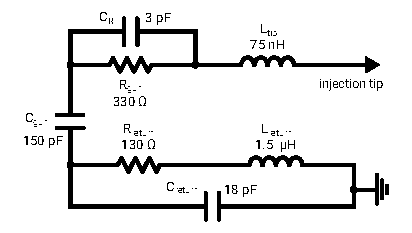
\includegraphics[width=0.3\textwidth]{src/1/figures/gun_model.pdf}
  \caption{ESD Gun model}
  \label{fig:esd-gun-model}
\end{figure}

% Explain the waveform
La forme d'onde est fournie dans la figure \ref{iec_pulse}.
Elle est définie pour une charge de 2\textOmega{}.
L'impulsion commence par un pic d'une largeur de $1ns$ risetime.
Il est suivi par une partie plus lente d'amplitude plus faible, mais qui dure plus longtemps (approximativement $200ns$).
Les niveaux de tensions peuvent atteindre 15kV et de courant 30A.

\begin{figure}[!h]
  \centering
  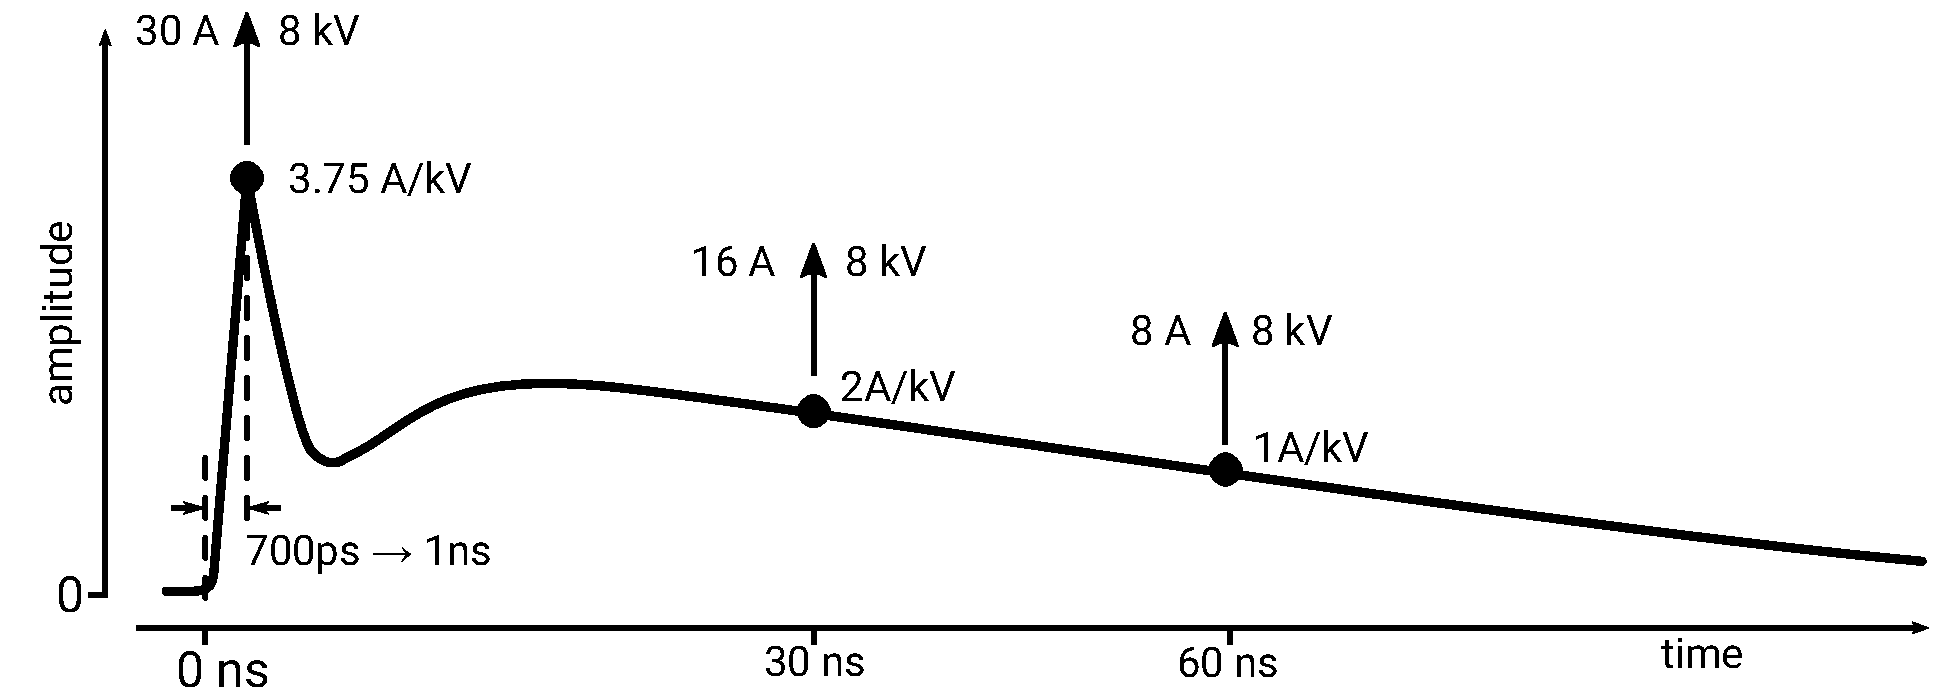
\includegraphics[width=\textwidth]{src/1/figures/iec61000-4-2_waveform.pdf}
  \caption{Main properties of an IEC 61000-4-2 pulse on a 2\textOmega\ resistive load}
  \label{iec_pulse}
\end{figure}

% autres méthodes
Il existe un grand nombre d'autres méthodes de test.
Dans l'automobile, le standard ISO 7637-2 est très largement employée pour qualifier les modules électroniques.
La méthode DPI (Direct Power Injection) est aussi très intéressante de par son circuit de couplage d'un stress sur une tension d'alimentation, ce qui est souvent nécessaire pour faire des tests ESD sur des produits en fonctionnement.

Une fois les produits testés, des cas de défaillances peuvent-être identifiés.
La partie suivante présente des cas de défaillances fonctionnelles trouvés dans la litterature.

\section{Méthodes d'analyse de faiblesses fonctionnelles}

%TODO
% Case 1 - NXP bandgap + substrate coupling
K. Abouda details in \cite{softfailEMCIC} a case of soft-failure on an integrated automotive regulator \gls{ic}.
The failure signature is a loss of the regulated voltage when exposed to \gls{bci} ISO11452-4 \cite{iso11452}.
The test setup is provided in Fig. \ref{}.
The product is investigated manually, by searching inside the design for coupling and propagation paths, and performing multiple simulations.
Eventually, it was proven that a residue of the disturbance was coupling through the substrate on a current mirror inside the bandgap reference.
During the disturbance, bandgap voltage was shifting from its nominal value.
After some delay, the bandgap output was reaching an undervoltage threshold, causing the entire system to restart.
To avoid it, a design fix was proposed by filtering at the appropriate spot inside the design to avoid the amplification of the disturbance.

\begin{figure}[!h]
  \centering
  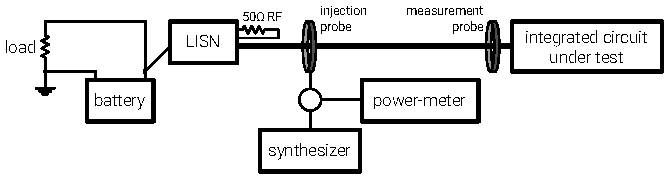
\includegraphics[width=\textwidth]{src/1/figures/bci_setup.pdf}
  \caption{Bulk Current Injection setup}
  \label{fig:bci-setup}
\end{figure}

% Case 2 - CESAME IC - paper Vrignon + Ben dhia
N. Lacrampe presents another failure case in \cite{LacrampeTransientImmunity}.
Very-fast \gls{tlp} is injected on an 0.18 \textmu{}m CMOS technology (1.8 V supply voltage) testchip.
The chip contains 6 instances on the same logic core, differing only by their power-rails architecture.
The injection on power rails is performed using a \gls{dc} block 1 nF capacitor, similarly to the \gls{dpi} standard \cite{iec62132-4}.
% What is the failure signature
An output signal of the logic core is monitored.
The susceptibility criteria is the amplitude crossing a 20\% threshold from the established logic level.
Above this threshold, the core is supposed to no longer work reliably.
It is proven that modelling the output buffer of the core logic is enough for reproducing with less than 20\% error the waveform on the output.
It is less accurate than a full-netlist simulation, but faster to simulate.
VHDL-AMS and \gls{spice} modelling are performed in this analysis.

%TODO: Pictures
% Case 3 - failures on an SDRAM
%TODO: Read reference articles in this article
In \cite{SDRAMCase}, soft-failures are studied on a SDRAM memory in operation.
The injection setup consists of a modified compact \gls{tem} cell \ref{fig:modified-tem-cell} with a reduced septum height.
Reduced dimensions result in increased field strenghts, to reach levels normally produced by an \gls{esd} gun.
The discharge waveform, injected inside the cell, is generated by a filtered \gls{tlp} and is similar in shape to IEC 61000-4-2 \cite{iec61000-4-2}.
The SDRAM chip is mounted on a board.
Data is written and read on the memory by \gls{fpga}.
Differences between incoming and outgoing data signifies a functional failure of the memory.
Only the memory is exposed to the disturbance, the rest of the board's devices are located outside of the \gls{tem} cell, on the other side of the board.
The main defect of this method is to only provide a global failure level.
It does not allow to identify which particular net or pin is the most sensitive to disturbances.

\begin{figure}[!h]
  \centering
  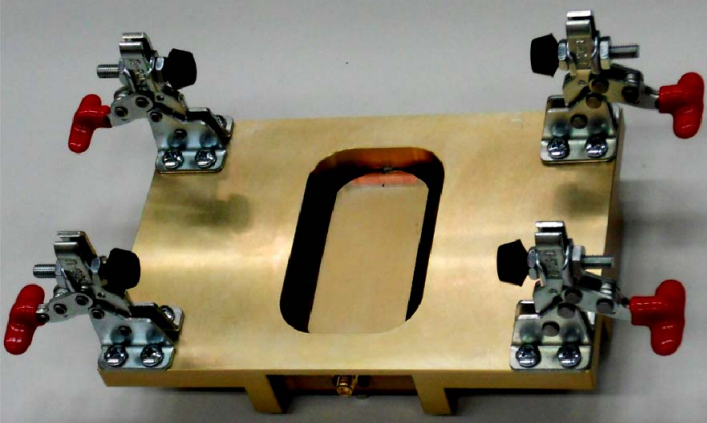
\includegraphics[width=0.6\textwidth]{src/1/figures/modified_tem_cell.png}
  \caption{Modified TEM cell from \cite{SDRAMCase}}
  \label{fig:modified-tem-cell}
\end{figure}

B. Orr reports in \cite{softFailSubsystem} errors caused by electrostatic discharges on two different camera communication buses.
Events of different severities are observed, depending on the discharge parameters.
It is attempted to determine whether the sensor or the application processor is causing the error.
The magnetic emission map is recorded with a near-field magnetic scanner to try to observe local variations in the emission spectrum because of the degradation of functionnality.
It was envisionned that soft-failure can induce significant variations in the emission spectrum of a disturbed component, and thus those variations could help localize them.
In this particular case, the root cause of failures could not be determined.

An LCD display is studied in \cite{softFailLCD}.
The device is tested with an IEC 61000-4-2 \cite{iec61000-4-2} generator, and non-destrutive problems are observed due to the discharge.
Electromagnetic disturbances cause stripes to appear on the display, optical parameters changes and blacklighting malfunctions.
System-level testing waveforms were found too complex for identifying the root cause.
A near-field injection is performed to identify which trace of the LCD's flex connector claims the lowest immunity.
The lack of resolution of the near-field probe caused multiple traces to be disturbed at once, preventing this second approach to work.
Finally, the individual track stressing was repeated with a capacitively-coupled \gls{tlp} on each individual metal track.
However, results were once more unconclusive and no metal trace could categorically be identified as more sensitive than the others.
The conclusion for this paper is that silicon level soft-error models are required for standard investigation.

An investigation method is presented in \cite{softFailMobile} to search for discharge propagation paths responsible for soft-failures on a mobile phone.
The IEC 61000-4-2 standard is chosen as testing waveform.
Metallic parts are assumed to be the main propagation paths.
To confirm this hypothesis, time-domain electromagnetic field 3D simulations of almost the entire phone are ran (see Fig. \ref{fig:mobile-phone-3d-em})
After the failure location was determined, RC-networks are used as countermeasures to protect physical inputs and outputs, like buttons, LCD inputs and connectors.

\begin{figure}[!h]
  \centering
  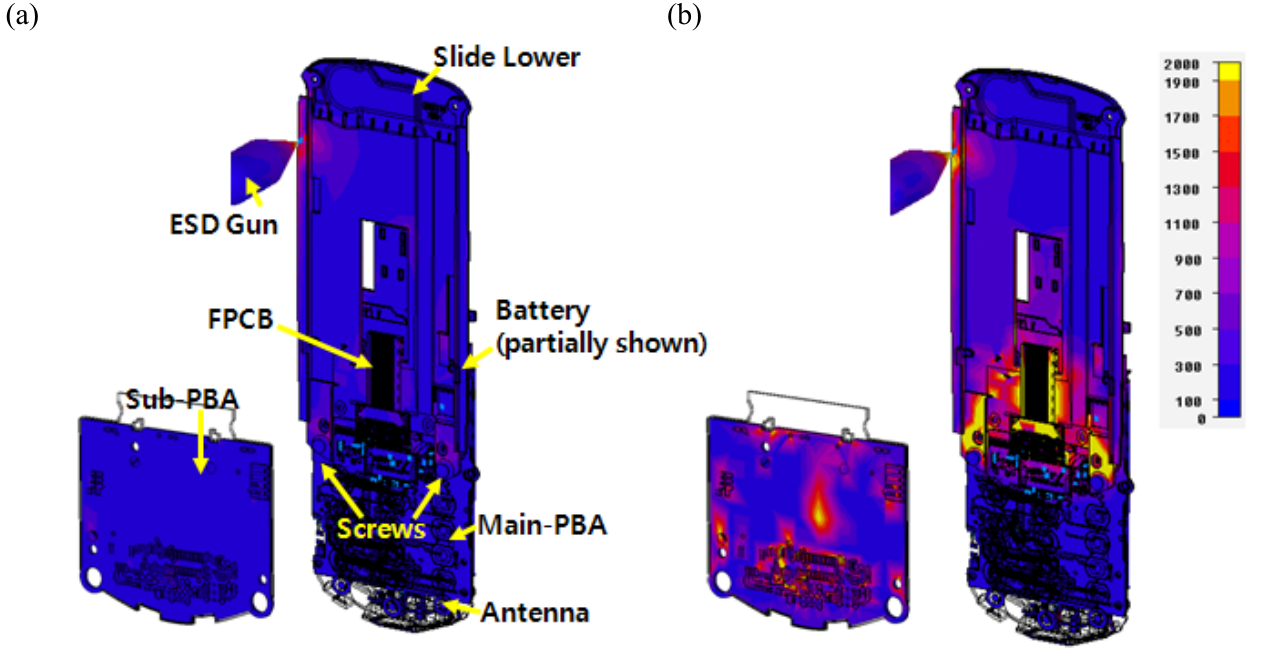
\includegraphics[width=0.8\textwidth]{src/1/figures/current_distribution_mobile.png}
  \caption{ESD Current Distribution on Mobile Phone and Backside sub-battery pack at (a) 1.0 ns and (b) 1.8 ns (Credit: \cite{softFailMobile})}
  \label{fig:mobile-phone-3d-em}
\end{figure}


Near-field scan

% Introduce near-field scanner
Electromagnetic near-field scanner measure maps of electric and magnetic field.
An electric or magnetic probe is swept closely above a device to record the emitted field in near-field conditions.
Measurements may be carried out in the frequency domain or in the time domain.
This tool was initially intended for architectural analysis such as floor-planning and power distribution analysis.
For ESD, spatial information provided by the recorded map is very useful to locate failures and malfunctions.
A comprehensive and detailed analysis of near-field antennas is done by A.D. Yaghjian in \cite{nfsFirstStudy}.
More recent work details the principle of operation, data processing and hardware requirements in \cite{near-field-scan, planarNFSAntenna, NFSMeasurements, NFScanner}.
Finally, measurement of electromagnetic emissions with surface scan method is standardized in IEC TS 61967-3 \cite{iec61967}.
The architecture of a near-field scanner is given in Fig. \ref{fig:near-field-scanner}.

\begin{figure}[!h]
  \centering
  \includegraphics[width=0.4\textwidth]{src/1/figures/architecture_near_field_scanner.pdf}
  \caption{Architecture of a near-field scanning testbench}
  \label{fig:near-field-scanner}
\end{figure}

\begin{figure}[!h]
  \centering
  \includegraphics[width=0.4\textwidth]{src/1/figures/near_field_scanner_susceptibility_map.pdf}
  \caption{Susceptibility map of a board recorded with surface scan in injection configuration \cite{}}
  \label{fig:near-field-scan-map}
\end{figure}

Revue des méthodes de modélisation

In the litterature, various ESD modelling methods can be found.
They comprise a wide range of techniques such as 3D electromagnetic and semiconductor physics simulations, compact, behavioral, physically-based and non-linear modelling.
The methods described hereafter could be used for soft-failure investigation.

M. Scholz details a mixed-mode ESD simulation approach in \cite{mixedModeESDSims}.
It is a combination of \gls{spice} and \gls{tcad} models, simulated in \gls{spice} environment.
The author indicates that the combination of physical device models and standard simulations provides higher accuracy and more realistic simulations than behavioral \gls{spice} models.
Using this complex simulation tool, on-chip and off-chip device interactions are studied, in powered and unpowered conditions.

In \cite{usb2ESDProtection}, TLP characterizations serves as an I(V) model for both external protections and an \gls{ic} pin.
The \gls{pcb} S-parameters are extracted from the board layout, using Momentum software (Agilent Technology).
It is electrically model with lumped R,L,C,G elements.
The modelling approach proved successful for simulation interactions between external devices and on-chip structures.
This method is interesting for soft-failure analysis because it is thorough and complete and enables accurate ESD simulation.

% IBIS is not enough for modelling an IC pin for ESD simulations
The Input Output Buffer Information Specification (IBIS) \cite{ibis-spec} is a behavioral, black-box model for performing signal integrity simulation on digital circuits.
It is widespread in the digital \gls{asic} world because it enables accurate simulations without disclosing circuit or process information.
It was envisionned that IBIS models could also be used or extended for ESD.
It is demonstrated in \cite{ibisImprovementFabrice} that the model lacks some parameters for EMC and ESD simulations.
It comprises a current versus voltage characteristic of \gls{io}s, similar to what can be extracted by a TLP, however the IBIS model is not defined for fast impulses and high injection.

N. Lacrampe proposes in \cite{LacrampeTransientImmunity} to perform 3D electromagnetic simulations at silicon level, using the integrated circuit layout, to deduce the amount of capacitive couplings between Vdd and Vss rails.
The extraction is performed with HFSS software (Ansoft).
The goal of this analysis is to predict the susceptibility of integrated circuits against electrostatic discharges.
\gls{pcb} tracks are modeled by a distributed RLC network.
The package data from the IBIS model \cite{ibis-spec} was used in the simulations.
Finally, a TLP stress generator is modelled using a lookup table I(V) component, in series with a 50\textOmega{} resistor.

Once again, electromagnetic fullwave simulations are conducted in powered-on ESD analysis in \cite{softFailMobile}.
System-level components are simulated, such as PCB, metallic casing and battery back.
3D EM simulations helps to identify the main discharge paths and locate the failure.
